\section{Технический проект}
\subsection{Общая характеристика организации решения задачи}

Необходимо спроектировать и разработать web-платформу для поиска работы, которая должна способствовать эффективному взаимодействию между соискателями и работодателями на рынке труда.

Платформа представляет собой набор взаимосвязанных электронных страниц, сгруппированных по разделам, содержащих текстовую, графическую и мультимедийную информацию (например, описания вакансий, резюме, изображения). Платформа размещается в Интернете по уникальному доменному имени, например, www.jobplatform.ru. Каждая страница платформы — это документ, созданный с использованием современных технологий веб-разработки (PHP, CSS, JavaScript и других).

\subsection{Обоснование выбора технологии проектирования}

На сегодняшний день информационный рынок, поставляющий программные решения в выбранной сфере, предлагает множество продуктов, позволяющих достигнуть поставленной цели – разработки web-платформы.

\subsubsection{Описание используемых технологий и языков программирования}

В процессе разработки web-сайта используются программные средства и языки программирования. Каждое программное средство и каждый язык программирования применяется для круга задач, при решении которых они необходимы.

\subsubsection{Фреймворк PHP (Symfony)}

Symfony — это высокопроизводительный фреймворк, основанный на языке программирования PHP, предназначенный для создания серверной части (backend) web-приложений. PHP используется для написания сценариев, которые исполняются на сервере и формируют динамические страницы платформы, такие как списки вакансий, личные кабинеты и результаты поиска. Symfony предоставляет мощные инструменты для работы с базами данных, обработки запросов через REST API и обеспечения безопасности (например, JWT-аутентификация).

\paragraph{Достоинства фреймворка Symfony}

Основные преимущества Symfony включают:

\begin{enumerate}
	\item Модульная структура, упрощающая масштабирование и поддержку кода.
	\item Встроенные механизмы валидации форм и управления пользователями, что идеально для реализации регистрации, авторизации и обработки резюме/вакансий.
	\item Интеграция с ORM (например, Doctrine) для удобной работы с базой данных (MySQL/PostgreSQL).
	\item Высокая производительность и поддержка современных стандартов PHP.
\end{enumerate}


\subsubsection{Язык программирования JavaScript (Vue.js)}

JavaScript — объектно-ориентированный язык программирования, используемый для создания интерактивных интерфейсов на стороне клиента. В рамках проекта применяется фреймворк Vue.js, который расширяет возможности JavaScript для построения динамического и divisions (e.g., Vue.js) фронтенда платформы. Vue.js позволяет создавать отзывчивый и интерактивный интерфейс, включая формы для резюме, фильтры поиска и карточки вакансий, без необходимости перезагрузки страницы.

Основные преимущества Vue.js:

\begin{enumerate}
	\item Компонентный подход, упрощающий разработку модульных интерфейсов (например, карточки вакансий, формы отклика).
	\item Реактивное обновление данных, обеспечивающее плавное взаимодействие (например, обновление списка вакансий при изменении фильтров).
	\item Лёгкая интеграция с REST API (Symfony) для получения данных с сервера.
	\item Кросс-браузерная совместимость, минимизирующая проблемы с отображением в разных браузерах.
\end{enumerate}

\subsubsection{MySQL}

MySQL — это реляционная СУБД с открытым исходным кодом, которая сочетает высокую производительность, простоту и масштабируемость. Она идеально подходит для веб-приложений, таких как платформы для поиска работы, где требуется быстрое и надёжное управление данными пользователей, резюме и вакансий. MySQL работает на всех популярных платформах и легко интегрируется с облачными сервисами, такими как AWS, Google Cloud и Azure.

Преимущества MySQL:

\begin{enumerate}
	\item Высокая производительность: Оптимизирована для быстрой обработки запросов, особенно в веб-приложениях с большим числом транзакций.
	\item Масштабируемость: Поддерживает горизонтальное и вертикальное масштабирование через репликацию и кластеризацию.
	\item Интеграция: Совместима с веб-фреймворками (Django, Laravel), NoSQL (MySQL Document Store) и платёжными системами.
	\item Надёжность: Транзакции (InnoDB) и репликация обеспечивают целостность данных.
	\item Поддержка сообщества: Обширная документация и активное сообщество разработчиков.
\end{enumerate}

Ограничения:

\begin{enumerate}
	\item Менее эффективна для сложных аналитических запросов по сравнению с PostgreSQL.
	\item Требует оптимизации для работы с очень большими базами данных.
\end{enumerate}

\subsection{Архитектура программной системы}

Диаграмма компонентов описывает физическую архитектуру web-платформы для поиска работы. Она иллюстрирует структуру системы, определяя зависимости между программными компонентами, включая исходный и исполняемый код.

На рисунке \ref{dc:image} изображена архитектура программной системы.

\begin{figure}[ht]
\center{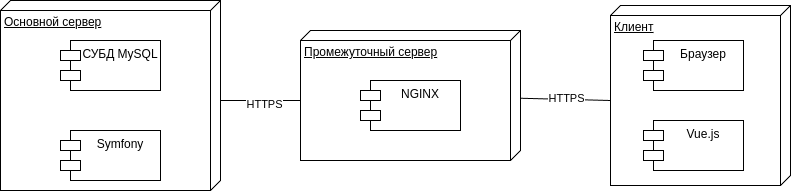
\includegraphics[width=1\linewidth]{dc}}
\caption{Архитектура программной системы}
\label{dc:image}
\end{figure}

Программно-информационная система состоит из следующих компонентов:

\begin{enumerate}
	\item Клиентская часть представлена устройством пользователя (ПК, смартфон или планшет), на котором установлен веб-браузер (например, Chrome, Firefox, Safari). В браузере работает Vue.js Frontend — клиентское приложение, обеспечивающее пользовательский интерфейс платформы. Через интерфейс пользователи (соискатели и работодатели) могут регистрироваться, создавать и редактировать резюме или вакансии, выполнять поиск по вакансиям/резюме и отправлять отклики. Взаимодействие между клиентской частью и сервером осуществляется по защищённому протоколу HTTPS, что гарантирует безопасность передачи данных, таких как личная информация пользователей и их действия на платформе.
	\item Промежуточный сервер реализован с использованием Nginx, который выполняет роль связующего звена между клиентской частью и основным сервером.
	\item Основной сервер реализован с использованием фреймворка Symfony, который отвечает за обработку запросов от клиентской части через REST API. Symfony обеспечивает бизнес-логику платформы, включая:
	
	\begin{itemize}
		\item управление пользователями.
		\item обработку данных о вакансиях и резюме.
		\item поиск и фильтрацию.
		\item обработку откликов на вакансии.
	\end{itemize}
	
	Для хранения данных используется СУБД MySQL, интегрированная с Symfony через ORM Doctrine, что упрощает управление данными и обеспечивает высокую производительность.
\end{enumerate}

\subsection{Структура базы данных}

Сущности и отношение между таблицами базы данных отражены на
рисунке \ref{bd:image}

\begin{figure}[H]
	\center{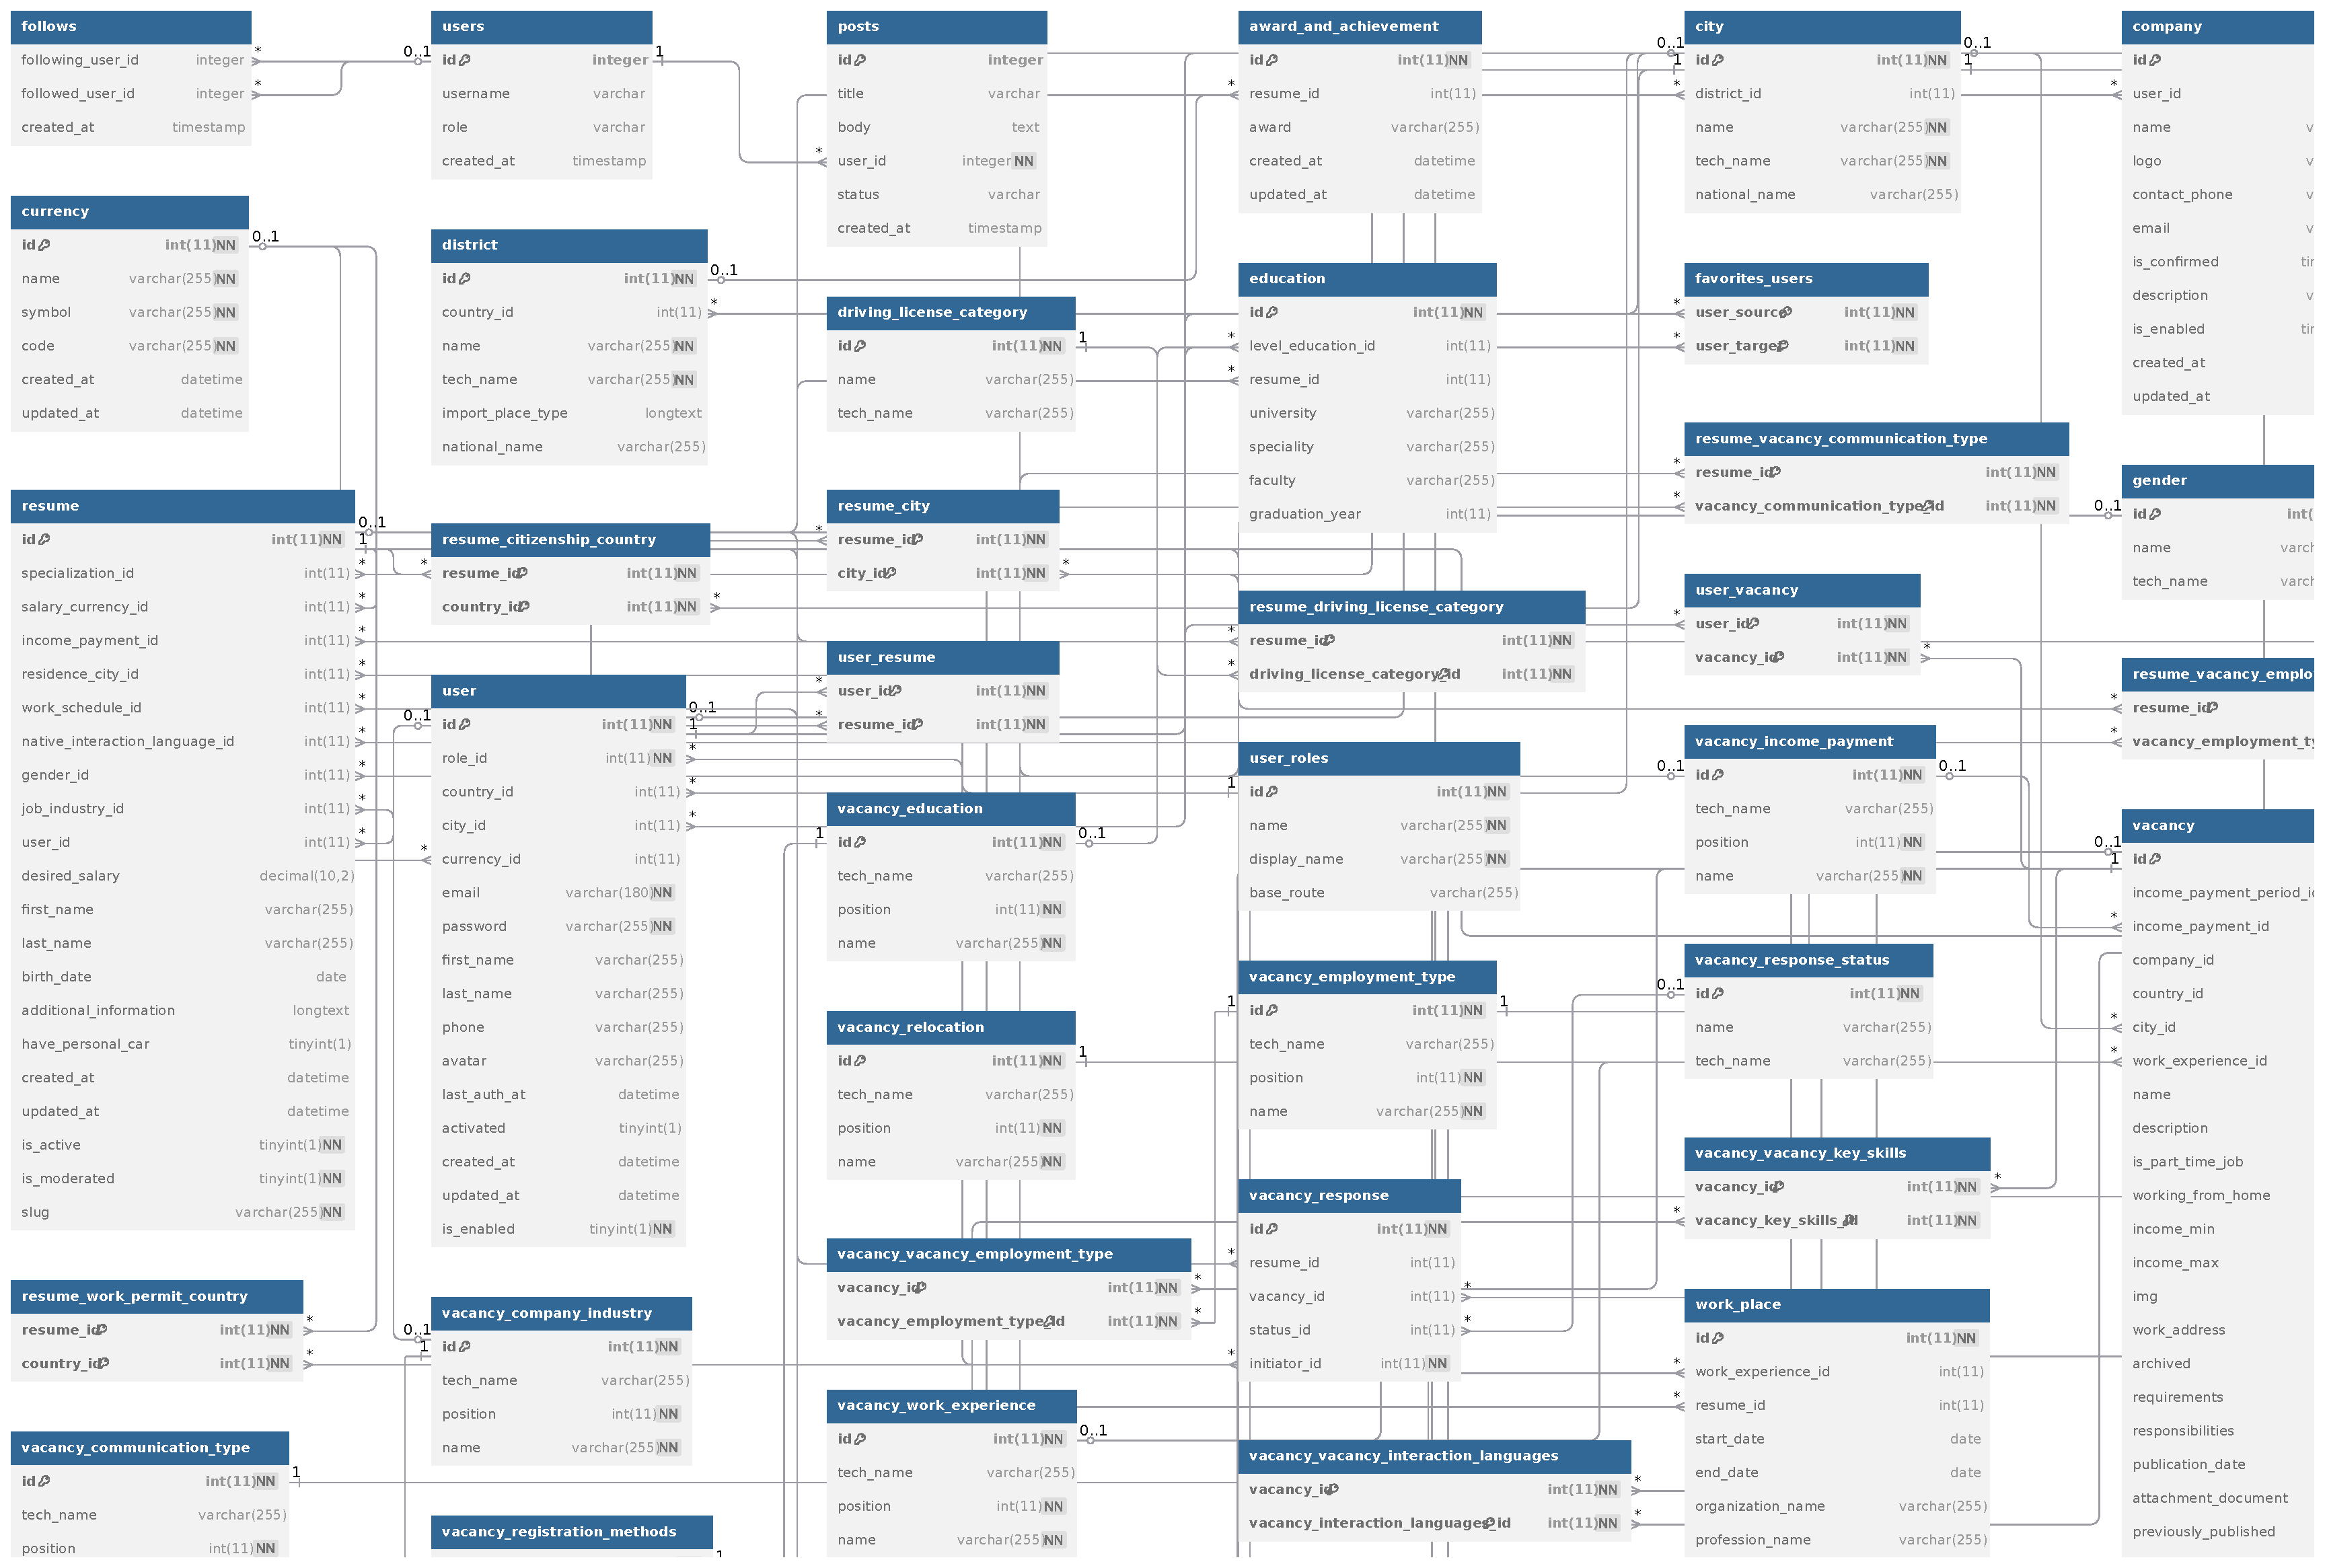
\includegraphics[width=1\linewidth]{bd}}
	\caption{ER-диаграмма}
	\label{bd:image}
\end{figure}


В таблице \ref{ssevsws:table} представлена структура таблицы resume.

\begin{xltabular}{\textwidth}{|l|l|p{1.7cm}|X|}
	\caption{Таблица resume \label{ssevsws:table}}\\ \hline
	\centrow Тип ключа & \centrow Имя столбца & \centrow Тип
	данных & \centrow Обязательность \\ \hline
	\thead{1} & \thead{2} & \centrow 3 & \centrow 4 \\ \hline
	\endfirsthead
	\continuecaption{Продолжение таблицы \ref{ssevsws:table}}
	\thead{1} & \thead{2} & \centrow 3 & \centrow 4 \\ \hline
	\finishhead
	primary key & id & integer & true \\ \hline 
	foreign key & specialization & integer & true \\ \hline 
	 & desiredSalary & string & true \\ \hline 
	 & firstName & string & true \\ \hline 
	 & lastName & string & true \\ \hline 
	 & birthDate & date & true \\ \hline 
	 & workPlace & string & false \\ \hline
	 & education & string & false \\ \hline
	foreign key & employmentType & integer & true \\ \hline
	foreign key & user & integer & true \\ \hline
\end{xltabular}

В таблице \ref{vacancy:table} представлена структура таблицы vacancy.

\begin{xltabular}{\textwidth}{|l|l|p{1.7cm}|X|}
	\caption{Таблица vacancy \label{vacancy:table}}\\ \hline
	\centrow Тип ключа & \centrow Имя столбца & \centrow Тип
	данных & \centrow Обязательность \\ \hline
	\thead{1} & \thead{2} & \centrow 3 & \centrow 4 \\ \hline
	\endfirsthead
	\continuecaption{Продолжение таблицы \ref{vacancy:table}}
	\thead{1} & \thead{2} & \centrow 3 & \centrow 4 \\ \hline
	\finishhead
	primary key & id & integer & true \\ \hline 
	 & name & string & true \\ \hline 
	foreign key & specializations & integer & true \\ \hline 
	& description & string & true \\ \hline 
	& incomeMin & string & true \\ \hline 
	& icomeMax & string & true \\ \hline 
   foreign key & incomePayment & integer & true \\ \hline
	foreign key & company & integer & true \\ \hline
	& requirements & string & false \\ \hline
	& responsibilities & string & false \\ \hline
	foreign key & city & integer & true \\ \hline
	foreign key & country & integer & true \\ \hline
	foreign key & employmentType & integer & true \\ \hline
\end{xltabular}

В таблице \ref{user:table} представлена структура таблицы user.

\begin{xltabular}{\textwidth}{|l|l|p{1.7cm}|X|}
	\caption{Таблица vacancy \label{user:table}}\\ \hline
	\centrow Тип ключа & \centrow Имя столбца & \centrow Тип
	данных & \centrow Обязательность \\ \hline
	\thead{1} & \thead{2} & \centrow 3 & \centrow 4 \\ \hline
	\endfirsthead
	\continuecaption{Продолжение таблицы \ref{user:table}}
	\thead{1} & \thead{2} & \centrow 3 & \centrow 4 \\ \hline
	\finishhead
	primary key & id & integer & true \\ \hline 
	& email & string & true \\ \hline 
	foreign key & roles & integer & true \\ \hline 
	& password & string & true \\ \hline 
	& firstName & string & true \\ \hline 
	& lastName & string & true \\ \hline 
	& phone & string & true \\ \hline
	foreign key & country & integer & false \\ \hline
	foreign key & companies & integer & false \\ \hline
	foreign key & vacancyFavorites & integer & false \\ \hline
	foreign key & resumeFavorites & integer & false \\ \hline
	foreign key & resumes & integer & false \\ \hline
	foreign key & favoriteUsers & integer & false \\ \hline
\end{xltabular}

В таблице \ref{company:table} представлена структура таблицы company.

\begin{xltabular}{\textwidth}{|l|l|p{1.7cm}|X|}
	\caption{Таблица vacancy \label{company:table}}\\ \hline
	\centrow Тип ключа & \centrow Имя столбца & \centrow Тип
	данных & \centrow Обязательность \\ \hline
	\thead{1} & \thead{2} & \centrow 3 & \centrow 4 \\ \hline
	\endfirsthead
	\continuecaption{Продолжение таблицы \ref{company:table}}
	\thead{1} & \thead{2} & \centrow 3 & \centrow 4 \\ \hline
	\finishhead
	primary key & id & integer & true \\ \hline 
	foreign key & user & integer & true \\ \hline 
	& name & string & true \\ \hline 
	& contactPhone & string & false \\ \hline 
	& email & string & false \\ \hline 
	& description & string & false \\ \hline
	foreign key & vacancies & integer & false \\ \hline
\end{xltabular}

В таблице \ref{country:table} представлена структура таблицы company.

\begin{xltabular}{\textwidth}{|l|l|p{1.7cm}|X|}
	\caption{Таблица vacancy \label{country:table}}\\ \hline
	\centrow Тип ключа & \centrow Имя столбца & \centrow Тип
	данных & \centrow Обязательность \\ \hline
	\thead{1} & \thead{2} & \centrow 3 & \centrow 4 \\ \hline
	\endfirsthead
	\continuecaption{Продолжение таблицы \ref{country:table}}
	\thead{1} & \thead{2} & \centrow 3 & \centrow 4 \\ \hline
	\finishhead
	primary key & id & integer & true \\ \hline 
	& name & string & true \\ \hline 
	& techName & string & true \\ \hline 
	foreign key & districts & string & false \\ \hline 
\end{xltabular}

В таблице \ref{district:table} представлена структура таблицы district.

\begin{xltabular}{\textwidth}{|l|l|p{1.7cm}|X|}
	\caption{Таблица vacancy \label{district:table}}\\ \hline
	\centrow Тип ключа & \centrow Имя столбца & \centrow Тип
	данных & \centrow Обязательность \\ \hline
	\thead{1} & \thead{2} & \centrow 3 & \centrow 4 \\ \hline
	\endfirsthead
	\continuecaption{Продолжение таблицы \ref{district:table}}
	\thead{1} & \thead{2} & \centrow 3 & \centrow 4 \\ \hline
	\finishhead
	primary key & id & integer & true \\ \hline 
	& name & string & true \\ \hline 
	& techName & string & true \\ \hline 
	foreign key & country & string & false \\ \hline 
	foreign key & cities & string & false \\ \hline 
\end{xltabular}

В таблице \ref{city:table} представлена структура таблицы city.

\begin{xltabular}{\textwidth}{|l|l|p{1.7cm}|X|}
	\caption{Таблица vacancy \label{city:table}}\\ \hline
	\centrow Тип ключа & \centrow Имя столбца & \centrow Тип
	данных & \centrow Обязательность \\ \hline
	\thead{1} & \thead{2} & \centrow 3 & \centrow 4 \\ \hline
	\endfirsthead
	\continuecaption{Продолжение таблицы \ref{city:table}}
	\thead{1} & \thead{2} & \centrow 3 & \centrow 4 \\ \hline
	\finishhead
	primary key & id & integer & true \\ \hline 
	& name & string & true \\ \hline 
	& techName & string & true \\ \hline 
	foreign key & district & string & false \\ \hline 
\end{xltabular}
